\documentclass[a4paper, fleqn,report]{jsbook}

%\documentclass[xelatex,a4paper,precisetext,noautoxspacing]{bxjsbook}
%
%\usepackage{fontspec}
%\setjamainfont{ipam.ttf}
%\setjasansfont{ipag.ttf}
%\setjamonofont{ipag.ttf}

\usepackage[dvipdfm,dvipdfmx]{graphicx}

\usepackage{amsmath,amssymb,amsfonts}
\usepackage{bm}
\usepackage{siunitx}

\usepackage[dvipdfmx, colorlinks=true, bookmarks=true,
bookmarksnumbered=true, bookmarkstype=toc, linkcolor=blue,
urlcolor=blue, citecolor=blue]{hyperref}
\usepackage{pxjahyper}

\setlength{\textheight}{592pt}
\setlength{\textwidth}{430pt}
\setlength{\oddsidemargin}{20pt}


\renewcommand{\maketitle}{%
\begin{titlepage}
 \null \vskip5em% ページ上部の空白t
 \begin{center}
  {\huge XX専攻XXコース修士学位論文} \vskip5em
  {\huge 格納容器熱水力挙動の数値解析} \vskip25em
  {\Large 2025年2月} \vskip1.5em
  {\Large 学籍番号XX    XX XX} \vskip1.5em
  %   {\LARGE  } \vskip2em
 \end{center}%
\end{titlepage}}


\begin{document}

\maketitle

%\begin{abstract}
 abstract
\end{abstract}

%% 目次
\tableofcontents
\listoffigures
\listoftables

%%%%%%%%%%%%%%%%%%%%%%%%%%%%%%%%%%%%%%%%%%%%%%%%
%%%  本文
%%%%%%%%%%%%%%%%%%%%%%%%%%%%%%%%%%%%%%%%%%%%%%%

\chapter{序章}
\section{背景}

図\ref{fig:log}に示す。

\begin{figure}[htbp]
    \centering
    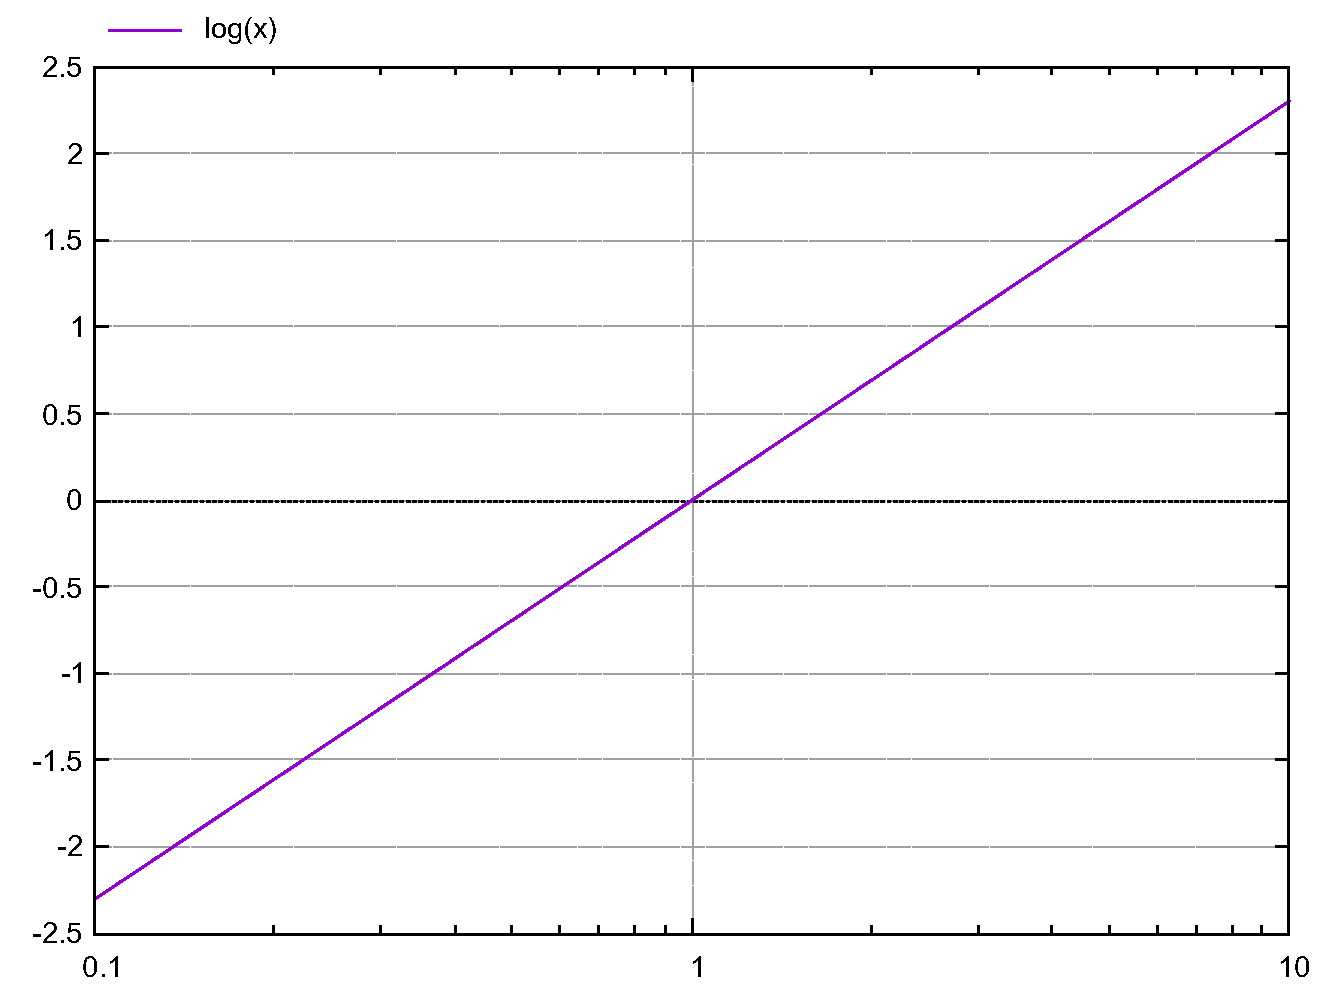
\includegraphics[scale=0.5]{Fig/log-fig.pdf}
    \caption{図のキャプション}
    \label{fig:log}
\end{figure}

\begin{table}[htbp]
    \centering
     \caption{実験条件}
    \begin{tabular}{cc}
    項目     &  内容 \\\hline
    ケース1     & 乱流 \\
    ケース2  &  層流 \\\hline
    \end{tabular}
       \label{tab:condition}
\end{table}
\chapter{解析手法}
\label{chap:simulation}

\section{はじめに}
陰解法を用いた場合,行列の反転,すなわち連立一次方程式を解く必要がある.
連立一次方程式の解法には直接法と反復法がある.直接法では厳密に解が求めら
れるが,計算量が多い.反復法は反復計算により近似解を求める方法であり,係
数行列の特性に応じて,高速に解を得られることがある.
CFDでは反復法が多く用いられる.行列の特性によって収束の速度に違いが出る
と考えられるので,各手法を適用し,最適なものを選択する.ここでは次の式で
表される$n$次元の連立一次方程式を解くことを考える.
\begin{equation}
 A\bm{x}=\bm{b}
\label{eq:linear}
\end{equation}
$A$は$n\times n$の係数行列,$x$は$n\times1$の解ベクトル,$b$は
$n\times1$のベクトルを表す.

この章では主に文献\cite{test1}を参考にした.
\section{直接法}
連立1次方程式を行列演算によって直接解く,直接法であるガウスの消去法につ
いて述べる.
\subsection{ガウスの消去法}
ガウスの消去法は.係数行列$A$を一度上三角行列に変形し,それから単位行列
$I$を求めることで解を得る.

ガウスの消去法による演算量は$O(n^3)$に比例して増大するため,次元の大きな
連立方程式を解くのは非現実的となる.このためCFDでは反復法が多く用いられ
る.

\section{反復法}
反復法では,初期値として適当な値を与え,真の解に収束する近似解を反復計算により求める.ただし,係数行列
によっては反復計算が収束せず,解を得ることができない場合がある.反復解が
収束するためには係数行列が対角優位であることが必要である.対角優位とは,
行列の対角成分が他の成分に比べて,その絶対値が大きいような行列である.
\begin{equation}
 |a_{ii}|>\sum_{i\neq j}|a_{ij}|, \;\;(i=1,...,n)
\end{equation}
ここで$a_{ij}$は係数行列の要素.


\section{反復法}
反復法では,初期値として適当な値を与え,真の解に収束する近似解を反復計算により求める.ただし,係数行列
によっては反復計算が収束せず,解を得ることができない場合がある.反復解が
収束するためには係数行列が対角優位であることが必要である.対角優位とは,
行列の対角成分が他の成分に比べて,その絶対値が大きいような行列である.
\begin{equation}
 |a_{ii}|>\sum_{i\neq j}|a_{ij}|, \;\;(i=1,...,n)
\end{equation}
ここで$a_{ij}$は係数行列の要素.


\chapter{解析結果}
\section{テスト1の結果}
本節では,テスト1の解析結果について示す。
\chapter{結論}



%% reference
\begin{thebibliography}{99}
\bibitem{test1} reference
%\bibitem{test2} reference
%\bibitem{test3} reference
%
\end{thebibliography}


\appendix
\chapter{付録1}

\end{document}

